


\begin{figure}
\small
    \centering
    \begin{minipage}[c]{.445\linewidth}
    \centering
    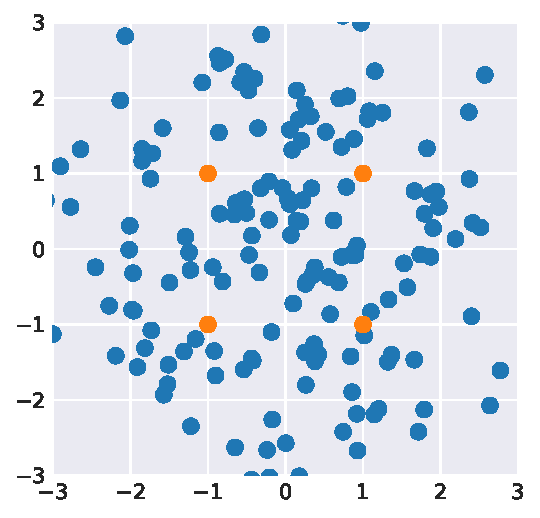
\includegraphics[width=.49\linewidth,clip,trim=0 0 5 0]{./assets/toy_example_2d/2d_toyexample_px_py.pdf}
    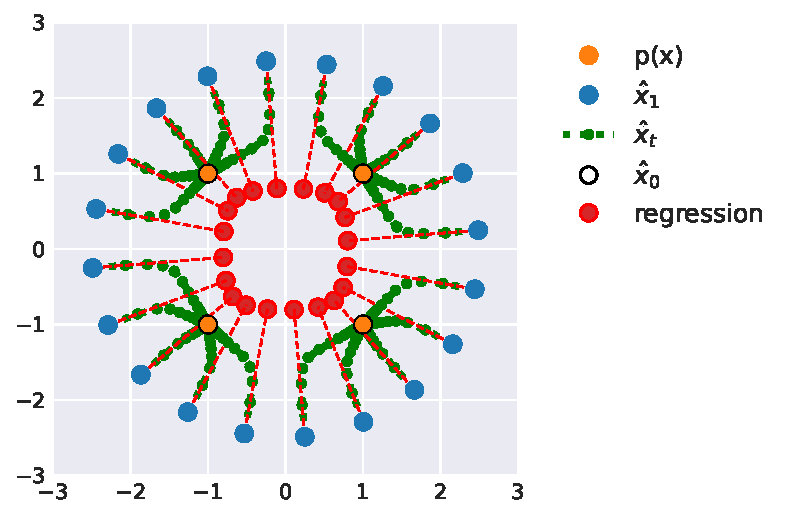
\includegraphics[width=.49\linewidth,clip,trim=0 0 125 0]{./assets/toy_example_2d/2d_toyexample_estim_large_radius.pdf}
    
    (a) 
    \end{minipage}
    \begin{minipage}[c]{.09\linewidth}
    \centering
    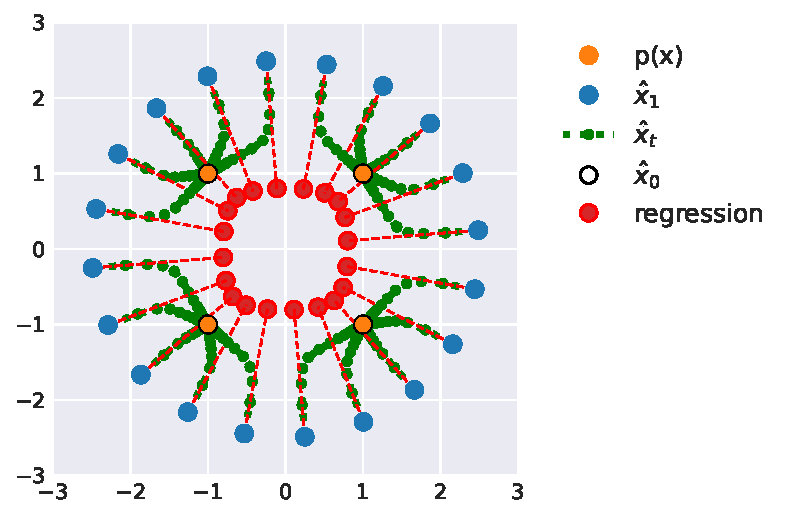
\includegraphics[width=\linewidth,clip,trim=260 0 10 0]{./assets/toy_example_2d/2d_toyexample_estim_large_radius.pdf}

    \end{minipage}
    \begin{minipage}[c]{.445\linewidth}
    \centering
    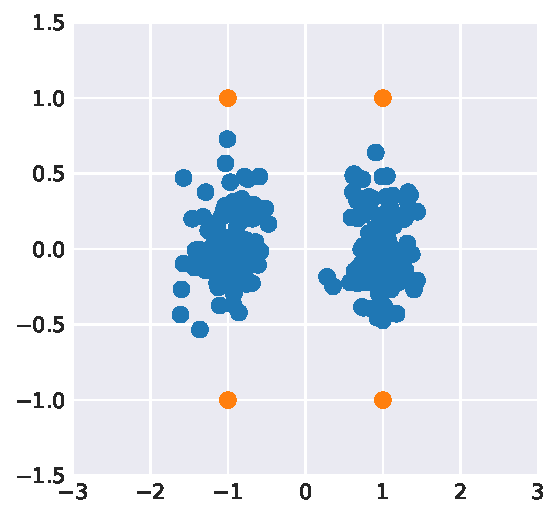
\includegraphics[width=.49\linewidth,clip,trim=0 0 5 0]{./assets/toy_example_2d/2d_toyexample_H_px_py.pdf}
    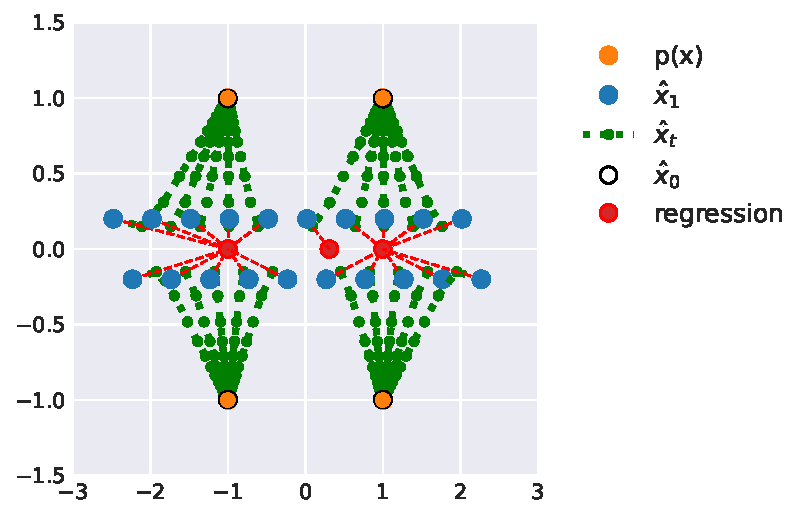
\includegraphics[width=.49\linewidth, clip, trim=0 0 125 0]{./assets/toy_example_2d/2d_toyexample_H_estim_large_radius.pdf}
    
    (b) 
    \end{minipage}

    \caption{2D Toy Example. Estimation of conditional mean and iterated estimation for points from a multimodal (4 modes) distribution under: (a) Denoising strong Gaussian noise ($\mH = \mI$); and (b) missing information recovery, i.e., $\mH=[1, 0; 0, 0]$, under moderate noise. Blue points represent observed samples, while red ones are the \emph{regression} prediction. The black (hollow) circles represent the final point in our iterative procedure, always reaching a valid point in the data manifold (orange points). The small green circles indicate the iterative restoration path.}
    \label{fig:2d_toy_example}
\end{figure}